\documentclass[11pt,letterpaper]{article}
\usepackage{array}
\usepackage[in]{fullpage}
\usepackage{verbatim}
\usepackage{parskip}
\usepackage{graphicx}
\usepackage{enumitem}
\usepackage{wrapfig}

\usepackage{titlesec}
\titlespacing{\section}{0pt}{\baselineskip}{0pt}
\titleformat*{\section}{\normalsize\bfseries\MakeUppercase}

\titlespacing{\subsection}{0pt}{0.5\baselineskip}{0pt}
\titleformat*{\subsection}{\normalsize\bfseries}

\titlespacing{\subsubsection}{0pt}{0.5\baselineskip}{0pt}
\titleformat*{\subsubsection}{\normalsize\bfseries}

%\setlength{\parindent}{0in}
\setlength\intextsep{0pt}

\begin{document}
\setlength{\parindent}{0in}
%\baselineskip 4pt
\newcommand{\tablespace}[0]{\vspace{8pt}}
\textbf{ENVS S422: Earth's Climate System\\
Modeling Exercise 5: Growth and decay of ice sheets}\\%\footnote{Based on exercises developed by Dave Bice at Penn State University.}}\\

In this exercise, you will do some experiments with a simple ice sheet model based on a classic paper by Johannes Weertman, from 1976. Our goals are to understand some basic things about how these ice sheets grow and shrink, and how they can respond to sunlight variations related to orbital changes of the Earth relative to the
Sun.

%\begin{figure}[b!]
%\begin{center}
%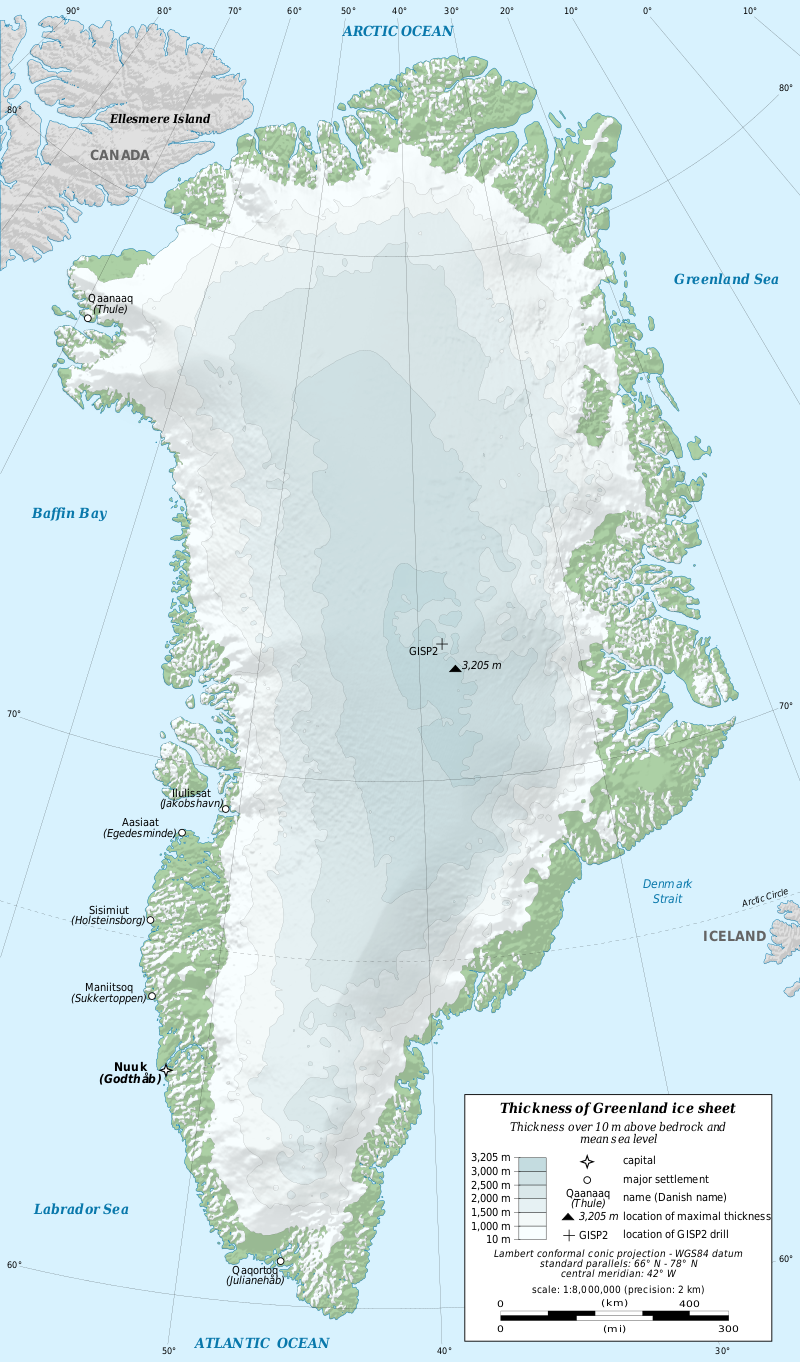
\includegraphics[width=3in]{./greenland.png}
%\end{center}
%\end{figure}

Large continental ice sheets such as Greenland are important components of the global climate system that play a critical role in altering the planetary albedo, which is connected to a potent positive feedback mechanism, and also in controlling the level of global sea level. Their growth and decline has been one of the dominant features of the Pleistocene glaciation, and their current decline is of great importance to the rising global sea level. The timing of the ice ages and intervening warmer periods are largely controlled by orbital changes, and one of the goals of this modeling exercise is to see how this works.

For each model experiment, you should submit a brief 1-paragraph response to the questions that are being explored in the exercise and \textit{at least} one graph to help justify your response.

Due date: 20 March 2019

\section{Model description}
\begin{wrapfigure}{r}{2.5in}
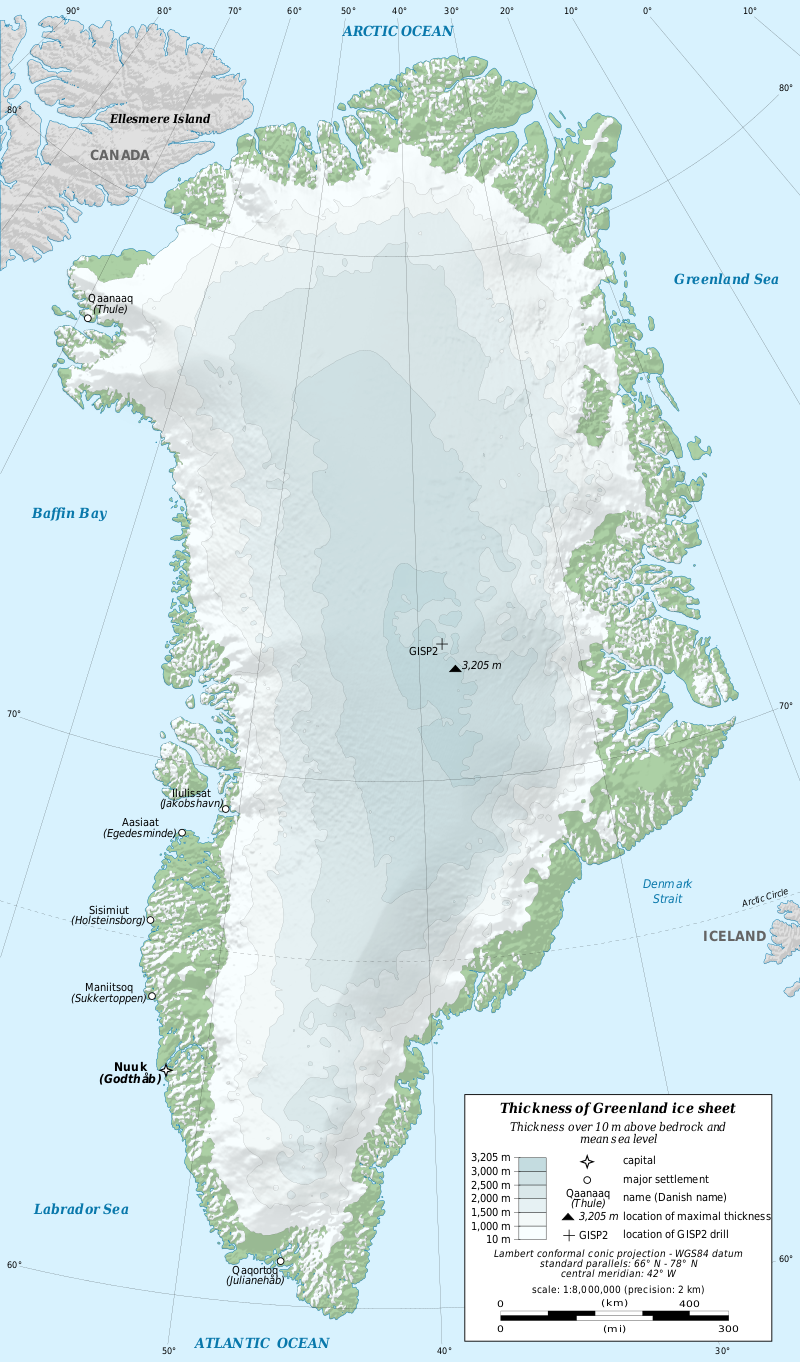
\includegraphics[width=2.5in]{./greenland.png}
\end{wrapfigure}
To develop our model of an ice sheet, we have to start with a few basics of how ice forms and flows. Glacial ice begins as snowfall that accumulates over the years. As it gets buried under more snow, the snow crystals undergo a kind of metamorphism, eventually turning into nearly solid ice. Ice, as a naturally occurring polycrystalline solid, is really a kind of rock. But unlike most other rocks, ice can actually flow at the surface without melting. This solid-state flow is quite fast relative to other geologic processes, enabling glaciers to be very dynamic features of the Earth's surface.

It is common to assume that ice behaves as a deformable plastic material, which means that there is a critical shear stress $\tau_0$ below which no strain (deformation or flow) will occur, and above which the strain is limitless. Stress is just a force acting on an area, and shear stress is a force applied parallel to a surface as opposed to a force applied perpendicular to a surface, which is called a normal stress. We talk about stresses rather than forces, since stresses are what can cause materials to deform (whether by flow or by fracture). The shear stress at the base of a column of ice, $\tau_b$, is given by\\
\begin{equation}
\tau_b = \rho g h \sin\alpha,
\end{equation}
where $\rho$ is ice density, $g$ is gravitational acceleration, $h$ is ice thickness, and $\alpha$ is the glacier surface slope. This means that thick ice with a shallow slope can have the same basal shear stress as thin ice with a steep slope. As the ice thins you need a higher slope to reach the critical shear stress. Considering that the height or thickness of the ice must taper to 0 at the glacier terminus, you can see that the slope of the glacier has to be greatest right at the edge (which is illustrated in a schematic way in the figure above).

\begin{figure}[]
\begin{center}
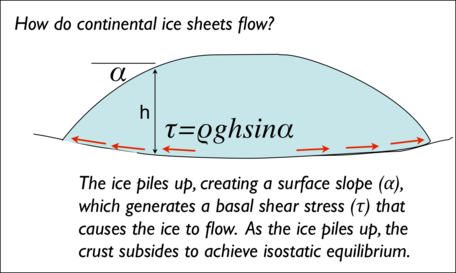
\includegraphics[]{./ice_sheet_flow_v2.png}
\end{center}
\end{figure}

If the slope is too low, the basal shear stress will not match the critical shear stress $\tau_0$, but as snow piles up, creating more ice, the slope will increase until $\tau_0$ is reached, at which point flow will begin. As flow begins, the slope will decrease; this causes the basal shear stress to drop below $\tau_0$ and flow will stop, but then snow piles up again and $\tau_0$ is met. Ultimately the glacier evolves to the point where the basal shear stress hovers right around the critical shear stress $\tau_0$ and a steady state condition occurs. The result of this is that a glacier has an equilibrium profile, which is described by 
\begin{equation}
h(x) =  \sqrt{\frac{2\tau_0}{\rho g}(L-|x|)} = \sqrt{\lambda(L-|x|)},
\label{eq:hx}
\end{equation}
where $L$ is the glacier length and $\lambda=2\tau_0/(\rho g)$. Note that the height $h$ is a function of position $x$, $x=0$ is the center of the ice mass (the so-called ``ice divide''). In your analysis, it will be useful to think about how the various parameters affect the ice thickness at the ice divide, which is
\begin{equation}
h(x=0) = \sqrt{\lambda L}.
\end{equation}
The ice sheet is considered to be perfectly symmetrical so that it looks the same in the $+x$ and $-x$ directions. Typical values for $\lambda$ are 8--15. The cross-sectional area is found by integrating Equation (\ref{eq:hx}) from $x=-L$ to $x=L$, which yields
\begin{equation}
A_x = \frac{4}{3}\lambda^{1/2}L^{3/2}.
\end{equation}
Rearranging to solve for $L$, we find that
\begin{equation}
L = \left(\frac{\left(\frac{3}{4}A_x\right)^2}{\lambda}\right)^{1/3}.
\end{equation}

The shape of the ice sheet, at two different times, is shown in the figure on the next page.
\begin{figure}
\begin{center}
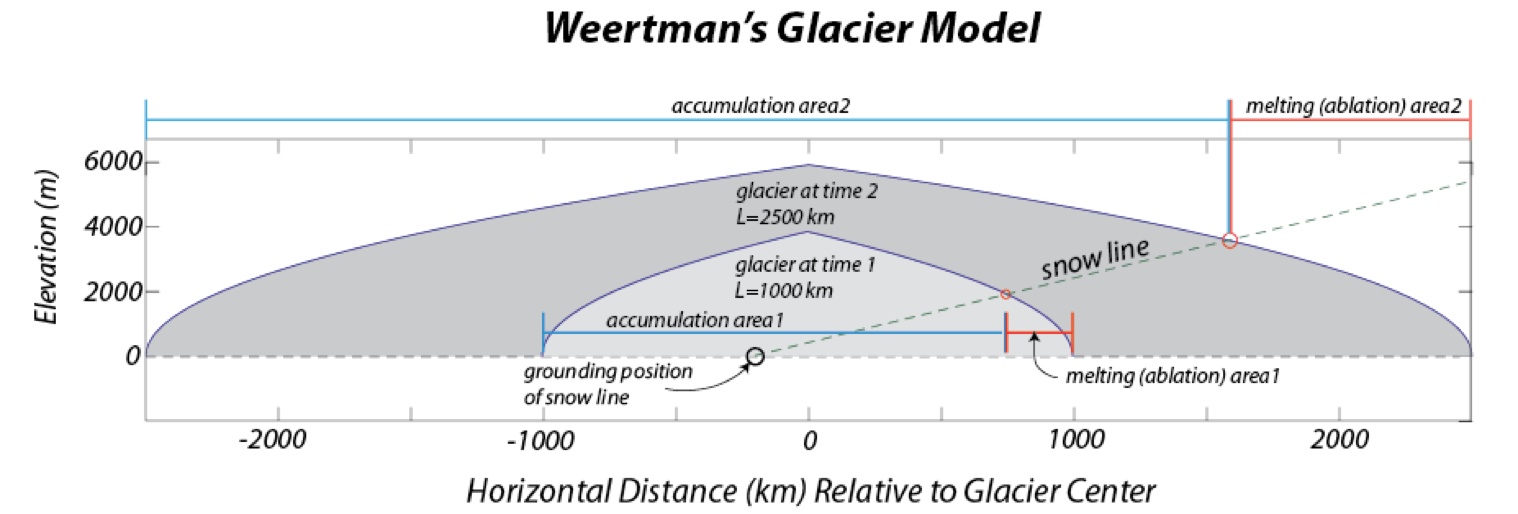
\includegraphics[width=\textwidth]{./weertmans_glacier_model_v2.png}
\end{center}
\label{fig:weertman}
\end{figure}

The figure also indicates the snow line, which separates colder areas where snow will accumulate to form ice from warmer regions where the melting exceeds snowfall and the glacier will experience a loss of ice. The snow line slopes gently up to the right towards the warmer side of the diagram. Where this snowline intersects the surface of the glacier (red circles above), we divide the glacier into its accumulation and melting (ablation) zones. The grounding position of the snowline (black circle above) marks the place where it intersects an elevation of zero. You can think of the $+x$ direction as indicating southern Greenland, and the $-x$ direction as indicating northern Greenland.

The model starts with an initial glacier length, and from that we can calculate the profile of the glacier and its cross-sectional area. Once we have the profile, we can find the intersection with the snow line, which allows us to separate the glacier into accumulation and ablation areas. We get the snow line by setting the equation for the snow line equal to the equation for the shape of the ice surface, which leads to a quadratic equation. Once we have the snow line, we can calculate the change in the cross sectional area as
\begin{equation}
\frac{dA_x}{dt}=L_{a}\dot b_{a}+L_{b}\dot b_{b},
\end{equation}
where $L_{a}$ and $L_{b}$ are the length of the accumulation and ablation areas $\dot{b}_{a}$ and $\dot{b}_{b}$ are the mean accumulation and ablation rates in the accumulation and ablation areas. Note that the ablation rate is negative. The net sum of accumulation and ablation then determines if the ice sheet will shrink or grow; in either case we assume that the ice sheet evolves slowly enough to maintain the equilibrium profile. In the model, the accumulation and ablation rates are related by a parameter epsilon, such that
\begin{equation}
\varepsilon=\frac{\dot{b}_{b}}{\dot{b}_{a}}
\end{equation}

If warming occurs, the ``grounding line'' (in this case, the spatial coordinate at which the snow line is at sea level) moves to the left ($‐x$ is considered to be toward the North), whereas cooling moves it to the South (right in the diagram). Based on observations of the present, Weertman calculated that the grounding position of the snowline changes by 17.7 km for every 1 W/m$^2$ of mean summer insolation change. In this way, we can make a connection between the orbitally-driven changes in summer insolation to the model as a way of forcing the glacier to grow and shrink.


\section{Experiments}

To begin with, make sure that the Milankovitch orbital variations of insolation are turned off so they do not impact the model.

\subsection{Steady State?  Response Time?\label{model:initial}}
In this first experiment, let’s see what happens to the glacier’s length over time with some reasonable initial conditions.

Time Specs:
\begin{itemize}
\item Run from -300,000 to 0 years, with a time step DT of 200 and using the Runge-Kutta 4 algorithm.
\end{itemize}
Model Parameters:
\begin{itemize}
\item accumulation\_rate = 1.2 \{m/yr\}
\item $\epsilon$ =  .24
\item initial\_grounding\_line = -400 \{km\}
\item initial\_length\_km = 400 \{km starting length\}
\item lambda = 14 \{ice strength parameter\}
\item slope = 0.002
\item Milank = 0 \{constant orbital forcing\}
\end{itemize}

\begin{enumerate}[label=(\alph*)]
\item Before running the model, try to predict what will happen to the ice sheet.  Will it find a steady state, or will it shrink to nothing or grow indefinitely?  Then run the model and explain what happens.

\item Now, change the initial length to 3000 km (a very large ice sheet).  Will it find a steady state again? How does your answer compare to what you found in (a)?  At the start, do you think that the net accumulation will be greater than or less than the net ablation?

\item How quickly does the ice sheet evolve toward its steady state? How fast does glacier grow/shrink?  In systems analysis, this is called the response time, and is often defined as the time it takes a system to accomplish about 2/3 of its change to the eventual steady state (so it really only applies to systems that tend toward a steady state). In the case of our glacier, you can find the difference in length between the steady state length and the starting length, and then find the point in time when about 2/3 of this change has been accomplished; that is your response time.

Use the model set-up and results from the first experiments (a \& b) to estimate the response time, giving the result in kyr.
\end{enumerate}

\subsection{Crossing the Threshold to Rapid Melting}

In the above experiment, you explored how the model results on were affected by two different initial lengths. Now, let’s explore a wider range of initial lengths, which will reveal an interesting change. Start with the same initial set-up as in \ref{model:initial}, where the initial length was 400 km. When doing these experiments you will want to make comparative graphs.

\begin{enumerate}[label=(\alph*)]
\item Run the model, and you should see the glacier grow to a length of about 2100 km and then level off, having reached a steady state.  

\item Decrease the initial length to 300 km.  What length does the glacier end up at?

\item Further decrease the initial length to 200 km. Now what length does the glacier end up at?  Describe, briefly, what happens to the glacier in this case.  Note that in (a), the rate of area/length change decreases as it approaches the steady state -- it gets there very gradually.  How does this deceleration of (a) compare with the behavior in this case?

\item Now increase the initial length to 210 km. What length does the glacier end up at? 

\item It should be clear to you that there is a threshold in the initial length that separates two very different behaviors and different outcomes.  Fiddle around with the initial length until you find the threshold (within 1 km is fine).
\end{enumerate}

\subsection{Changing the Grounding Line}

Now let’s see what happens if we change the position of the grounding line, which is shown graphically below, shifted to the left (towards more negative values). Shifting the grounding line 
\begin{figure}[b]
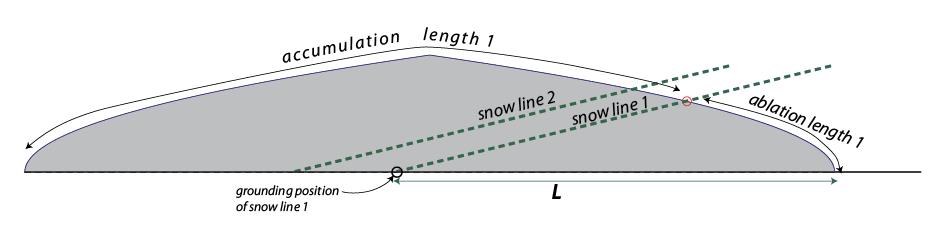
\includegraphics[width=\textwidth]{./grounding_line.png}
\end{figure}
is a crude way of imposing a warming of the glacier. 

\begin{enumerate}[label=(\alph*)]
\item Start with the same model set-up as in \ref{model:initial}. Run the model to act as a control, taking note of the ending length and the general behavior. Then shift the grounding line to -500 km.  Make a prediction about what will happen, then run the model and describe how this change affects the glacier.

\item Now shift the grounding line to -300 km and make a prediction about how this will affect the glacier, then run the model and describe how this change affects the glacier.
\end{enumerate}

\subsection{Changing the Ice Strength ($\lambda$)}

Now investigate the affect of changing the ice strength parameter ($\lambda$), which affects the critical shear stress for flow of the ice. Decreasing $\lambda$ effectively lowers the critical shear stress, making it easier for ice to flow. This would mean that ice can flow with a smaller thickness and/or surface slope. To begin, again use the standard set-up from \ref{model:initial}, which has $\lambda=14$. Run this ``control'' model first, and take note of the ending length and maximum thickness of the glacier. 

\begin{enumerate}[label=(\alph*)]
\item Change $\lambda$ to 12, thus making the ice flow more easily. Run the model and describe what happens. Did the glacier become longer/shorter relative to the control? How about its surface elevation?

\item Further reduce $\lambda$ to 10. Again, run the model and compare your results to the control.
\end{enumerate}


\subsection{Ratio of Accumulation and Ablation Rates ($\epsilon$)}

How will changing the ratio of accumulation and ablation rates affect the growth of the ice sheet?  The model parameter $\epsilon$ controls this ratio.  Again use the model set-up from \ref{model:initial} as the control, in which $\epsilon$ is set at 0.24. First run this model to recall what happens to the length. 

\begin{enumerate}[label=(\alph*)]
\item Now change $\epsilon$ to 0.28. Remember that the ablation rate is equal to the accumulation rate divided by epsilon. Run the model and describe what happens and why. How does changing epsilon to a larger value affect the ablation rate? How/why does that affect the equilibrium length of the glacier?

\item Now change epsilon to 0.20. Again, run the model and describe what happens and why.
\end{enumerate}


%\subsection{Changing the Slope of the Snowline}
%
%What will happen if the slope of the snowline increases?  It is already set to a very low value of 0.002.  First, let’s visualize what this would do to the glacier (see figure below). You can see that increasing the slope will shorten the accumulation length and increase the ablation length.  So, what will this do to the growth of the glacier?
% 
%As before, we begin with the model set-up for 1a, and then run this model to remind ourselves of the control case.  Take note of the beginning ablation length in the control.
%
%\begin{figure}[b]
%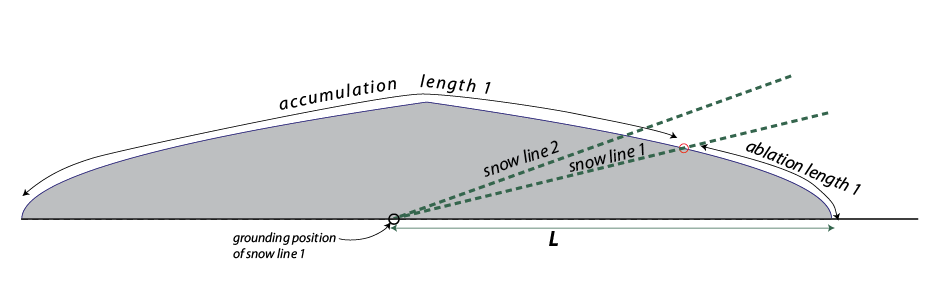
\includegraphics[width=\textwidth]{./climate_slope.png}
%\end{figure}
%
%
%\begin{enumerate}[label=(\alph*)]
%\item Change the slope slightly to 0.0022. Run the model and explain what happens and why.  How does the beginning ablation length of this model compare with the control?  How did the results compare with your prediction?
%
%\item Now increase the slope even more to 0.0024.  Run the model and describe what happens and why.
%\end{enumerate}


\subsection{Orbital Forcing}
Now, we will connect the orbital forcing to the model by turning on the Milank switch (by setting it equal to 1). Again, start with the initial model from \ref{model:initial}. Now, with the Milank switch turned on, the changing summer insolation due to orbital variations will force the grounding line position to move back and forth over time. Higher insolation pushes the grounding line position to the north (toward more negative values), while a decrease in insolation moves the grounding line to the south (toward more positive values). As you should know by now, moving the grounding line position will cause the glacier to advance and retreat.

Run the model and plot the length in km and Qt (the orbitally controlled variation in summer insolation), and study the relationship between the peaks and troughs in Qt and the size of the ice sheet.  

\begin{enumerate}[label=(\alph*)]
\item Study the relationship between the glacier’s length and Qt (the insolation over time).  Are they perfectly in sync, or does one seem to lag the other?

\item What is the lag time in kyr of the ice sheet relative to Qt?

\item How consistent is this lagtime?

\item What is the range of variation in the length of the glacier in km? For comparison, the Laurentide ice sheet expanded and contracted about 25$^\circ$ of latitude from it's center of mass ($x=0$) and there are 111 km per degree of latitude.

\item Now compare the ice sheet length with the SPECMAP record of del18O, which is partly a measure of ice volume and partly a measure of temperature -- higher values represent more ice and colder temperatures.  How well do they agree?  How similar or dissimilar are the timing of the peaks and troughs?

\item Look at the most recent 10 kyr of the model.  How is Qt changing during this time, and how does the model glacier respond?  What does this suggest might be happening at the present time if we were not increasing the greenhouse effect through elevated CO$_2$ levels --- entering another small glaciation or holding steady or moving to a warmer interglacial?
\end{enumerate}

\subsection{Feedback Loops}
Glacier evolution is determined by two fundamental feedback loops between climate and glacier geometry (length and width). One of these feedback loops is positive, the other is negative. Which one, length or width, forms a positive feedback loop with climate and which one forms a negative feedback loop. Why? Describe how the feedback loops operate.

\end{document}

